\graphicspath{ {project_images/} }
\section{Related Works}

\subsection{SVM}
The first algorithm we looked at was Support Vector Machine (SVM) Classifier. 
Initial Research done showed that SVM outperformed Naive Bayes when perfoming image classification \cite{SVM}.
Through the use of Pipeline and Grid Search, we were able to find optimal performing parameters including: kernel, C, and gamma.
Grid Search allowed us to perform K-Fold cross validation on the model so that we would obtain more stable results.

\subsection{CNN}
Convolutional Neural Networks (CNN) were the main types of algorithms used by others looking into Image Classification.
This is because previous studies have shown the advantages to using such models to analyze and predict based on such complex datasets \cite{CNNPerformance}.
Additionally, there are various works using CNN models to perform varying types of Image Classification for several animals including primates, rodents, canines, felines, aves, and insecta \cite{AnimalSpecies1, AnimalSpecies2, AnimalBreed, Mosquito}.
When constructing our CNN models, we used the ReLu activation function for each hidden layer as well as the Adam optimizer since this seemed to be a common practice to improve performance.

\subsection{VGG16}
ADD RELATED WORK HERE
ADD CITATION HERE TOO

\subsection{CLIP}
As a last experimental algorithm, we also used a recently developed algorithm called Contrastive Language-Image Pre-training (CLIP) from OpenAI, the creators of prominent AI development technologies \cite{CLIP}.
This algorithm is a pre-trained model on images that are encoded, as well as associated text that has also been encoded to match the image.
The advantage of using CLIP was to experiment by using a novel technique called Zero-Shot Prediction (ZSP).
ZSP is the notion of encoding an image as well as a list of text that is the target feature, and having the pre-trained model perform a prediction based on no training from your dataset.
In our case, the target feature was to determine the target animal within the image: cat, dog, or panda.

\begin{figure}[h]
	\centering
	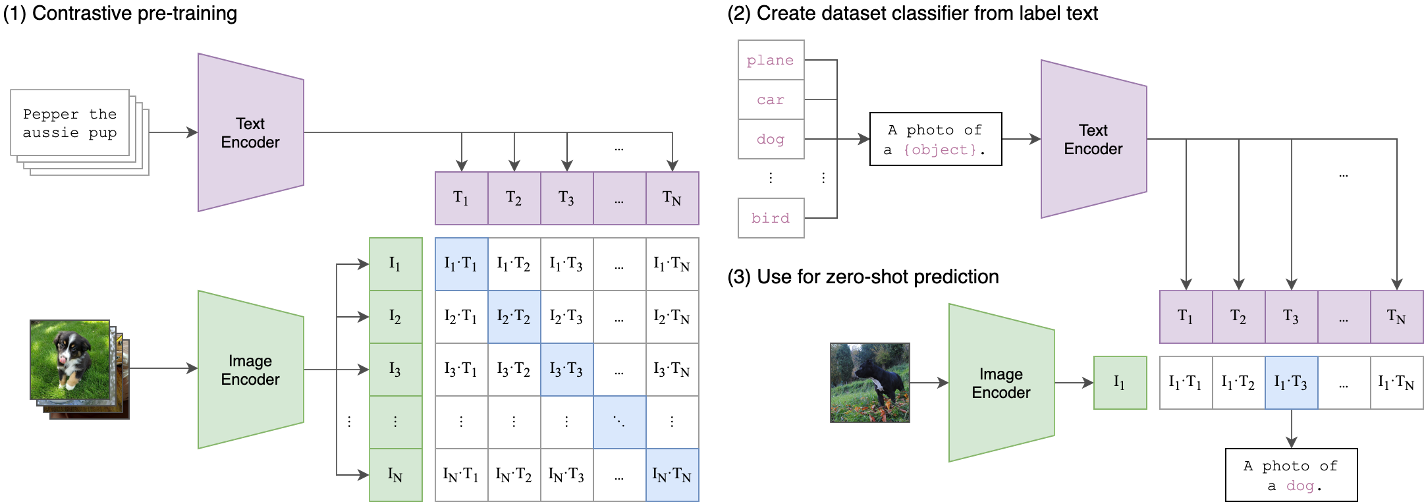
\includegraphics[scale=0.5]{CLIP_structure}
	\caption{CLIP model summary.}
	\label{fig:figure3}
\end{figure}

Because of the inability to change parameters and adjust the model, it will be excluded from the comparison to the other techniques.
The other algorithms used will be explained within the Methods section.

\subsection{Hypothesis}
Between the three animals, we expected to see Pandas being the most accurately predicted class since they are always Black and White, and have high contrast in fur.
This is especially true when compared to dogs and cats, which can come in a variety of colored fur.
Furthermore, we expected the Neural Network Algorithms as well as the pre-trained algorithms to perform faster and more accurately than SVM.